\documentclass{article}
\usepackage[utf8]{inputenc} 
\usepackage[T1]{fontenc}      
\usepackage[polish]{babel}
\usepackage[letterpaper,top=2cm,bottom=2cm,left=3cm,right=3cm,marginparwidth=1.75cm]{geometry}
\usepackage{amsmath}
\usepackage{graphicx}
\usepackage[colorlinks=true, allcolors=blue]{hyperref}
\renewcommand{\cftsecleader}{\cftdotfill{\cftdotsep}}

\title{Powiązanie zależności między tętnem a cyklem oddechowym przy użyciu sztucznej inteligencji
 }
\author{
    Bancerewicz Jan 198099 \\
    Kotłowski Julian 197694 \\
    Lozovyy Ostap 197747 \\
    Morawska Julia 198209 \\
    Rzęsa Mateusz 198417
}
\linespread{1.5}
\begin{document}
\maketitle
\newpage
\tableofcontents

\newpage

\section{Wprowadzenie i cel pracy}
Diagnostyka kardiologiczna często wykorzystuje metody sztucznej inteligencji, takie jak uczenie maszynowe czy sieci neuronowe, w procesie analizy sygnałów elektrokardiograficznych (EKG) czy fotopletyzmografii (PPG). Dzięki cyfrowemu przetwarzaniu sygnałów możliwe jest nie tylko wykrywanie subtelnych nieprawidłowości w pracy serca, a także monitorowanie kluczowych parametrów, takich jak zmienność rytmu serca (HRV).
Cyfrowa analiza sygnału EKG pozwala na zwiększenie czułości detekcji nieprawidłowości, trudnych do zauważenia w papierowych zapisach. Istotne  miejsce w owej analizie zajmują splotowe sieci neuronowe (CNN), które wykazują dużą skuteczność w klasyfikacji i wykrywaniu wzorców. 

Sygnał PPG rejestrowany za pomocą kamer smartfonów stanowi źródło informacji o przepływie krwi i stanie naczyń krwionośnych.
Integracja danych z EKG oraz PPG umożliwia uzyskanie pełniejszego obrazu stanu fizjologicznego pacjenta, co znacząco zwiększa skuteczność wykrywania arytmii oraz oceny reakcji organizmu na czynniki wewnętrzne i zewnętrzne.


\section{Założenia teoretyczne}
\subsection{EKG}
Elektrokardiografia (EKG) to metoda rejestracji aktywności elektrycznej serca poprzez powtarzające się cykle jego pracy. Pomiar dokonywany jest za pomocą elektrod umieszczonych w określonych miejscach na klatce piersiowej, ramionach lub nogach. Wykrywają one niewielkie zmiany potencjału elektrycznego towarzyszące skurczowi i rozkurczowi mięśnia sercowego.

\subsubsection{Załamki}
Elektryczna aktywność serca zostaje przedstawiona jako zapis liniowy, na którym widoczne są wzrosty i spadki na liniach nazywanych załamkami, oznaczane kolejno literami: P, QRS i T. Załamek P powstaje w momencie skurczu przedsionków i przepompowania krwi do komór serca. Następnie zespół QRS odzwierciedla skurcz komór serca wypełnionych krwią. Składa się on z trzech fal:
\begin{itemize}
\item \textbf{Załamek Q} odzwierciedla depolaryzację przegrody międzykomorowej, a jego obecność może mieć związek z fazą oddechu. 
\item \textbf{Załamek R} odpowiada za depolaryzację głównej masy mięśnia komór, co wiąże się z największym przepływem ładunku elektrycznego.
\item \textbf {Załamek S} oznacza końcową fazę depolaryzacji komór.
\end{itemize}
Załamek T ukazuje repolaryzacja komór umożliwiając ich rozluźnienie i przygotowuje je do kolejnego cyklu skurczu.

\subsubsection{Interwały RR}
W zapisie EKG czas pomiędzy kolejnymi uderzeniami serca najczęściej przedstawiany jest na podstawie odstępu między szczytami załamków R. Te wartości, określane jako interwały RR, są wyrażane w milisekundach (ms) i odzwierciedlają długość pojedynczego cyklu pracy serca. Na podstawie tych odstępów możliwe jest wyznaczenie tętna chwilowego, czyli częstotliwości rytmu serca w danym momencie. Wielkość ta definiowana jest jako stosunek liczby sekund w jednej minucie do długości aktualnego interwału RR wyrażonego w sekundach. Zmienność długości kolejnych interwałów RR stanowi podstawę analizy rytmu serca (HRV), która dostarcza informacji o funkcjonowaniu autonomicznego układu nerwowego.

\subsubsection{RMSSD}
RMSSD (Root Mean Square of Successive Differences), czyli pierwiastek kwadratowy ze średniej kwadratowej różnic czasowych między kolejnymi odstępami RR, jest wskaźnikiem aktywności przywspółczulnej części autonomicznego układu nerwowego. Dzięki odporności na długoterminowe zakłócenia RMSSD jest jednym z najczęściej stosowanych narzędzi w analizie krótkoterminowej zmienności rytmu serca HRV.

\subsection{HRV}
Zmienność rytmu serca (HRV) to zjawisko fizjologiczne polegające na zmianach odstępów czasu między kolejnymi uderzeniami serca, czyli różnicach w czasie pomiędzy szczytami załamków R w sygnale EKG. HRV jest mierzone poprzez analizę wahań tych odstępów. 

Podczas głębokiego oddychania obserwuje się, że rytm serca nie jest stały. Przy wdechu uderzenia serca stają się szybsze, natomiast wolniejsze przy wydechu. Zmienność odstępów między kolejnymi skurczami jest naturalnym zjawiskiem fizjologicznym, określanym jako oddechowa arytmia zatokowa, i stanowi oznakę prawidłowego funkcjonowania układu autonomicznego.

\subsubsection{Analiza HRV}
Do analizy częstotliwościowej HRV wykorzystuje się dwa zakresy:
\begin{itemize}
\item \textbf{Fale niskiej częstotliwości LF (0,04–0,15 Hz)} odzwierciedlają aktywność układu nerwowego odpowiedzialnego za reakcje organizmu w spoczynku i w stresie. Wzrost wartości LF występuje po zmianie pozycji ciała z leżenia do stania, gdy układ krążenia adaptuje się do nowego ułożenia. Zbliżony efekt występuje po głębokim wdechu lub podczas bardzo wolnego oddychania (poniżej 8,5 oddechu na minutę).

\item \textbf{Fale wysokiej częstotliwości HF (0,15–0,4 Hz)} są związane z aktywnością układu przywspółczulnego. Wzrost mocy pasma HF następuje podczas snu, relaksu, spokojnego oddychania oraz przy wydłużonym wydechu. Poziom HF bywa wyższy w nocy, co sprawia, że porównywanie go między porą poranną, dzienną i wieczorną może być niemiarodajne.

\end{itemize}

\newpage
Ocena zmienności rytmu serca powinna uwzględniać zarówno ogólne wskaźniki, takie jak SDNN, jak i parametry krótkoterminowe, np. RMSSD. W analizie częstotliwościowej szczególne znaczenie mają wartości mocy sygnału w pasmach niskoczęstotliwościowym oraz wysokoczęstotliwościowym.
Wyższe wartości tych parametrów są zazwyczaj interpretowane jako wskaźnik lepszej kondycji funkcjonalnej autonomicznego układu nerwowego. Szczególnie pożądana jest wysoka moc w paśmie HF, która odzwierciedla aktywność przywspółczulnego układu nerwowego. Z kolei przewaga aktywności w paśmie LF może sugerować dominację współczulnego układu nerwowego.


\subsection{PPG}
Fotopletyzmografia (PPG) to technika optyczna, służąca do monitorowania zmian objętości krwi w naczyniach krwionośnych, zwłaszcza zlokalizowanych w powierzchniowych warstwach tkanek, takich jak skóra. Umożliwia śledzenie pulsacji serca oraz przepływu krwi przez tkanki.

PPG wykorzystuje światło podczerwone o niskiej intensywności, emitowane przez diodę LED. Promieniowanie to przechodzi przez tkanki biologiczne lub odbija się od ich powierzchni, a następnie jest rejestrowane przez fotodiodę. Część światła ulega absorpcji przez skórę, kości oraz krew. W wyniku cyklicznych skurczów serca dochodzi do okresowych zmian objętości krwi w naczyniach, co powoduje zmienność w poziomie pochłanianego światła. W rezultacie czujnik PPG rejestruje rytmiczne zmiany intensywności sygnału świetlnego, umożliwiając uzyskanie sygnału odpowiadającego aktywności pracy serca.

\subsubsection{Składowe sygnału PPG}
Sygnał PPG składa się z dwóch głównych komponentów:
\begin{itemize}
\item \textbf{Składowa stała DC} reprezentuje optyczne właściwości tkanek, takich jak rozpraszanie światła oraz stałą objętość krwi żylnej i tętniczej. Zależna jest od budowy i struktury tkanek organizmu. Wykazuje niewielkie zmiany związane z cyklem oddechowym.
\item \textbf{Składowa przemienna AC} odzwierciedla zmiany objętości krwi tętniczej spowodowane pracą serca oraz zsynchronizowane z rytmem jego bicia dynamiczne wahania przepływu krwi. Wykazuje charakter cykliczny i zmienny w czasie, a oscylacje nakładają się na stabilniejszą składową sygnału DC.
\end{itemize}

\subsubsection{Analiza PPG}
Do ewaluacji zmienności składowej przemiennej sygnału PPG w czasie wykorzystuje się analizę widmową opartą na szybkiej transformacie Fouriera (FFT). Metoda ta pozwala na przekształcenie sygnału z dziedziny czasu do dziedziny częstotliwości, umożliwiając precyzyjną identyfikację częstotliwości odpowiadającej rytmowi serca. FFT jest przydatne w analizie sygnałów okresowych, ponieważ dekomponuje złożony sygnał na sumę fal sinusoidalnych, pozwalając na lokalizację tętna w widmie częstotliwościowym oraz ocenę jego zmienności.


\section{Charakterystyka zbioru danych}
Dane wykorzystane do trenowania i testowania modeli zostały pozyskane z wykorzystaniem czujnika Polar H10, który umożliwia rejestrację sygnału elektrokardiograficznego z częstotliwością próbkowania wynoszącą 130 Hz. Wysoka częstotliwość próbkowania umożliwia szczegółową analizę sygnału oraz precyzyjną detekcję załamków R.


W celu zgromadzenia odpowiedniego zbioru danych przeprowadzono dwugodzinne pomiary dla pięciu różnych osób. Rejestrowane sygnały różniły się między sobą w zależności od poziom aktywności fizycznej, rytm oddechu, zmienność rytmu serca (HRV), a także obecność nagłych ruchów ciała, które mogły wprowadzać zakłócenia.


Transmisja danych między czujnikiem a komputerem odbywała się bezprzewodowo z wykorzystaniem technologii Bluetooth Low Energy (BLE). Urządzenie identyfikowano na podstawie unikalnej nazwy. Dane były przesyłane w czasie rzeczywistym, w pakietach zawierających około 13 próbek zgodnie z zastosowaną częstotliwością próbkowania i zapisywane do plików w celu dalszej analizy. Każda próbka odpowiadała wartości napięcia elektrycznego rejestrowanego na powierzchni klatki piersiowej użytkownika.

\section{Przegląd zastosowanych metod}
Sieci neuronowe to zaawansowane modele stosowane w uczeniu maszynowym, inspirowane budową i działaniem ludzkiego mózgu, gdzie neurony są połączone w warstwy tworzące złożone struktury.

Jednym z najbardziej efektywnych rodzajów tych sieci jest konwolucyjna sieć neuronowa (CNN), przeznaczona głównie do przetwarzania danych o strukturze siatki, takich jak obrazy czy sygnały. CNN składa się z wielu specjalistycznych warstw, z których każda pełni określoną funkcję:
\begin{itemize}
    \item \textbf{warstwa konwolucyjna} wychwytuje istotne cechy z danych wejściowych, tworząc mapę cech.
    \item \textbf{warstwa aktywacyjna} wprowadza nieliniowość do działania sieci, pozwalającą lepiej modelować złożone zależności w danych.
    \item \textbf{warstwa normalizująca} redukuje rozmiar danych, co upraszcza dalsze przetwarzanie i zwiększa odporność modelu na zakłócenia.
    \item \textbf{warstwa spłaszczająca} przekształca dane z postaci wielowymiarowej w jednowymiarowy wektor.
    \item \textbf{warstwa w pełni połączona}  analizuje wyodrębnione cechy i dokonuje klasyfikacji na podstawie wzorców wykrytych w poprzednich warstwach.
    \item \textbf{warstwa wyjściowa} generuje końcowy rezultat działania sieci.
\end{itemize}

\begin{figure}[h]
    \centering
    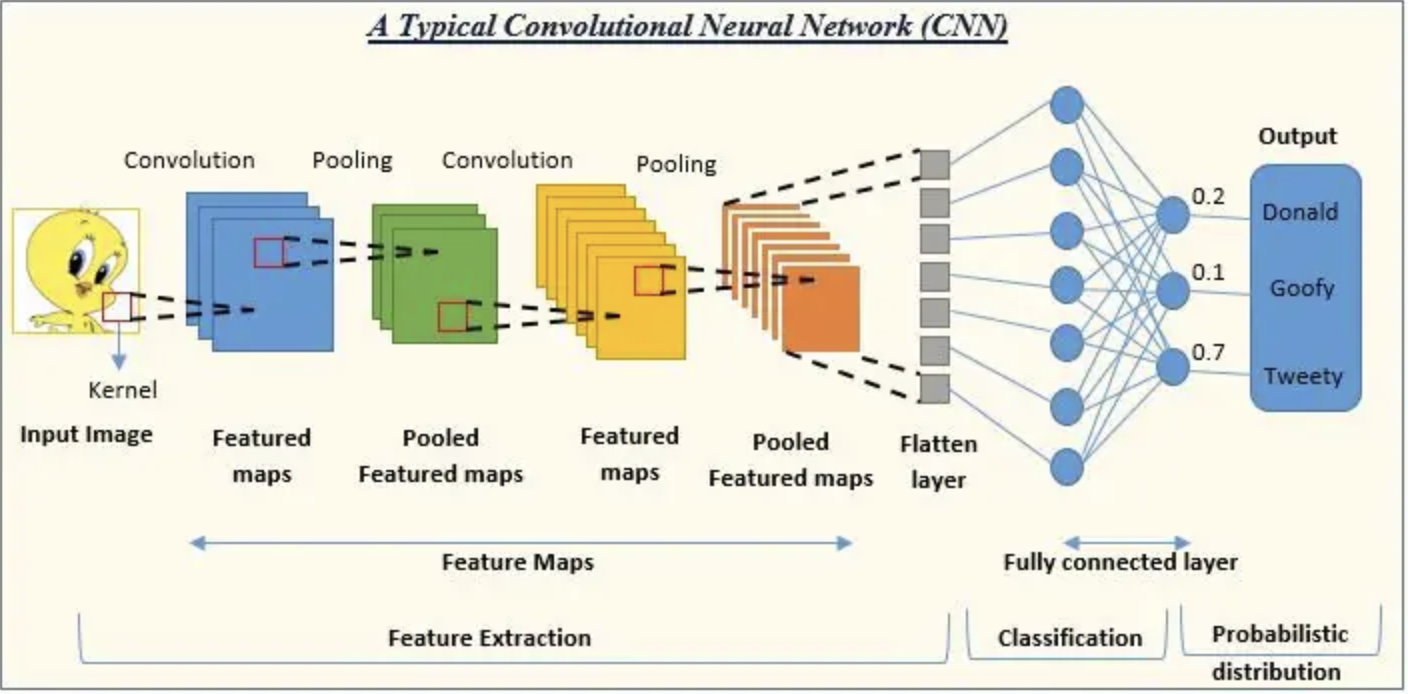
\includegraphics[width=0.7\textwidth]{Screenshot 2025-06-04 at 19.51.57.png}
    \caption{Wizualizacja konwolucyjnych sieci neuronowych}
\end{figure}
\subsection{Sieć do wykrywania R pików}
Model sieci neuronowej został zaprojektowany przy użyciu biblioteki PyTorch i dostosowany do analizy sygnałów elektrokardiograficznych (EKG). Przetwarzane dane mają formę jednowymiarowych sygnałów napięcia elektrycznego, podzielonych na fragmenty o długości 256 próbek.

Sieć opiera się na czterech warstwach konwolucyjnych 1D, które umożliwiają ekstrakcję cech z danych wejściowych. Każda z warstw zawiera normalizację grupową BatchNorm1d oraz funkcję aktywacji LeakyReLU. 

\begin{table}[h!]
\renewcommand{\arraystretch}{1.3}
\centering
\begin{tabular}{|c|c|c|c|c|}
\hline
\textbf{Warstwa} & \textbf{Kanały wejściowe} & \textbf{Kanały wyjściowe} & \textbf{Rozmiar filtru} & \textbf{Padding} \\
\hline
1 & 1   & 16  & 5 & 2 \\
2 & 16  & 32  & 5 & 2 \\
3 & 32  & 64  & 3 & 1 \\
4 & 64  & 128 & 3 & 1 \\
\hline
\end{tabular}
\caption{Parametry warstw konwolucyjnych}
\end{table}

\vspace{0.5cm}
Opis działania warstw:
\begin{itemize}
    \item Ekstrahuje podstawowe cechy z sygnału wejściowego, zwiększając liczbę kanałów do 16.
    \item Pogłębia reprezentację cech, rozszerzając ją do 32 kanałów.
    \item Wydobywa bardziej złożone wzorce z wcześniej przetworzonych danych, zwiększając liczbę kanałów do 64.
    \item Generuje końcową, bogatą reprezentację o 128 kanałach.
\end{itemize}
\newpage

Po każdej warstwie konwolucyjnej zastosowano operację maksymalnego próbkowania MaxPooling1d z jądrem o rozmiarze 2 i krokiem 2, co pozwala na stopniową redukcję wymiarowości danych wzdłuż osi czasowej i zwiększa efektywność przetwarzania.

W dalszej części modelu zastosowano jednokierunkową warstwę typu LSTM, której celem jest uchwycenie zależności czasowych w sygnale.

\begin{table}[h!]
\renewcommand{\arraystretch}{1.3}
\centering
\begin{tabular}{|l|p{10cm}|}
\hline
\textbf{Parametr} & \textbf{Opis} \\
\hline
Rozmiar wejścia & Warstwa LSTM przyjmuje dane wejściowe o wymiarze sto dwadzieścia osiem, co odpowiada liczbie kanałów wyjściowych uzyskanych z ostatniej warstwy konwolucyjnej i zapewnia zgodność strukturalną modelu. \\
\hline
Liczba jednostek ukrytych & W warstwie LSTM zastosowano sto dwadzieścia osiem jednostek ukrytych, co wynika z przyjęcia bazowej liczby sześćdziesięciu czterech i jej podwojenia w celu zwiększenia pojemności modelu. \\
\hline
Liczba warstw & Architektura zawiera jedną warstwę rekurencyjną, co pozwala ograniczyć złożoność modelu oraz ryzyko nadmiernego dopasowania do danych uczących. \\
\hline
Tryb przetwarzania danych & Dane wejściowe są przetwarzane w trybie, w którym pierwszy wymiar odpowiada liczbie próbek w partii, co jest wyrażone poprzez ustawienie parametru batch\_first na wartość True. Format danych przyjmuje postać: partia, długość sekwencji, liczba cech. \\
\hline
\end{tabular}
\caption{Opis parametrów warstwy LSTM zastosowanej w modelu}
\end{table}


Po przejściu przez warstwę LSTM, dane są spłaszczane i przekazywane do dwóch kolejnych, w pełni połączonych warstw liniowych.

\begin{table}[h]
    \centering
    \label{tab:fc_layers}
   \begin{tabular}{|c|c|c|}
        \hline
        \textbf{Warstwa} & \textbf{Rozmiar wejścia} & \textbf{Rozmiar wyjścia} \\
        \hline
        Liniowa 1 & liczba kroków czasowych $\times$ liczba jednostek LSTM & 128 \\
        \hline
        Liniowa 2 & 128 & 256  \\
        \hline
    \end{tabular}
        \caption{Struktura w pełni połączonych warstw liniowych po warstwie LSTM}
\end{table}


Wynikiem działania drugiej warstwy liniowej jest wektor o długości równej liczbie próbek w sygnale wejściowym. Każda wartość tego wektora jest logitem reprezentującym stopień pewności modelu, że w danej próbce występuje pik R w sygnale EKG.

\subsection{Sieć do obliczania RMSSD}
Model sieci neuronowej został zaprojektowany z wykorzystaniem biblioteki PyTorch. Został on dostosowany do estymacji parametru RMSSD na podstawie jednowymiarowych sekwencji odstępów RR, wyznaczonych z sygnału EKG i podzielonych na fragmenty o długości 10.

Model oparty jest na architekturze wielowarstwowego perceptronu, złożonego z czterech kolejnych warstw liniowych, których celem jest przekształcenie wektora wejściowego w pojedynczą wartość numeryczną.

\begin{table}[h!]
\renewcommand{\arraystretch}{1.3}
\centering
\begin{tabular}{|c|c|c|}
\hline
\textbf{Warstwa} & \textbf{Rozmiar wejścia} & \textbf{Rozmiar wyjścia} \\
\hline
Liniowa 1 & 10 & 64 \\
Liniowa 2 & 64 & 128 \\
Liniowa 3 & 128 & 64 \\
Liniowa 4 & 64 & 1 \\
\hline
\end{tabular}
\caption{Parametry warstw liniowych zastosowanych w modelu}
\end{table}

Opis działania warstw:
\begin{itemize}
    \item Przekształca 10-elementowy wektor odstępów RR w reprezentację o 64 cechach, umożliwiając pierwszą transformację nieliniową.
    \item Rozszerza przestrzeń reprezentacji do 128 wymiarów, pozwalając na modelowanie bardziej złożonych zależności.
    \item Redukuje liczbę neuronów do 64, wprowadzając kompresję informacji.
    \item Zwraca końcową estymację RMSSD jako pojedynczą wartość rzeczywistą.
\end{itemize}

Każda z warstw ukrytych zawiera funkcję aktywacji ReLU, która umożliwia sieci modelowanie nieliniowych zależności pomiędzy wartościami odstępów RR. 
Do nauki modelu wykorzystano średni błąd kwadratowy (MSE), który ocenia zgodność przewidywanych i rzeczywistych wartości RMSSD. Proces treningu realizowany był przy użyciu algorytmu optymalizacji Adam, charakteryzujący się stabilną konwergencją.

\newpage
\newpage
\begin{table}[h!]
\renewcommand{\arraystretch}{1.3}
\centering
\begin{tabular}{|l|p{10cm}|}
\hline
\textbf{Parametr} & \textbf{Opis} \\
\hline
Rozmiar wejściowy & Wektor zawierający 10 kolejnych odstępów RR w milisekundach \\
\hline
Funkcja aktywacji & Funkcja ReLU stosowana po każdej warstwie ukrytej w celu wprowadzenia nieliniowości \\
\hline
Funkcja straty & Wykorzystanie funkcji MSELoss do oceny jakości predykcji \\
\hline
Optymalizator & Algorytm Adam, który posiada szybkość uczenia równą 0{,}001 \\
\hline
Liczba epok treningowych & 500 \\
\hline
Rozmiar partii & 32 \\
\hline
\end{tabular}
\caption{Parametry i ustawienia procesu treningowego}
\end{table}

Dane treningowe przygotowano na podstawie 8 różnych sygnałów EKG, w których wcześniej wykryto piki R oraz obliczono wartości odstępów RR. Na ich podstawie wygenerowano sekwencje o długości 10, którym przypisano odpowiadające im wartości RMSSD. Aby zwiększyć liczbę dostępnych próbek, zastosowano technikę ruchomego okna, przesuwając je po sygnale. Model trenowano w sposób nadzorowany, wykorzystując pary wejście–etykieta.

\newpage
\section{Ewaluacja modeli}
\subsection{Sieć do wykrywania szczytów R}
W celu oceny skuteczności zaprojektowanej sieci neuronowej do wykrywania szczytów R przeprowadzono testy na niezależnym zbiorze danych, wykorzystując wytrenowane wcześniej wagi modelu. 

\begin{table}[h]
\centering
\begin{tabular}{|c|c|c|}
\hline
 & \textbf{Predykcja: brak szczytu R} & \textbf{Predykcja: szczyt R} \\
\hline
\textbf{Rzeczywiste: brak szczytu R} & 231170 & 53 \\
\hline
\textbf{Rzeczywiste: szczyt R} & 83 & 2678 \\
\hline
\end{tabular}
\caption{Macierz konfuzji dla klasyfikacji obecności szczytu R}
\end{table}

Na podstawie macierzy konfuzji wynika, że model poprawnie zaklasyfikował 231170 przypadków braku szczytu R oraz 2678 przypadków jego obecności. Liczba fałszywie pozytywnych klasyfikacji wyniosła jedynie 53, natomiast liczba fałszywie negatywnych 83.
Uzyskana wartość miary F1 wyniosła 0{,}9752, co wskazuje na bardzo dobrą równowagę pomiędzy precyzją a czułością modelu. 


\begin{table}[h]
\centering
\begin{tabular}{|l|c|p{9cm}|}
\hline
\textbf{Metryka} & \textbf{Wartość} & \textbf{Opis} \\
\hline
Skuteczność & 96{,}99\% & Model poprawnie określił obecność bądź brak szczytu R w sygnale EKG w niemal 97\% przypadków. \\
\hline
Błędne detekcje & 0{,}00\% & Model nie wygenerował żadnych fałszywych alarmów – nie rozpoznał piku tam, gdzie faktycznie go nie było. \\
\hline
Braki detekcji  & 3{,}01\% &Mmodel w około 3\% przypadków nie wykrył rzeczywistych szczytów R. \\
\hline
\end{tabular}
\caption{Wyniki działania modelu do wykrywania szczytów R}
\end{table}

Otrzymane wyniki potwierdzają wysoką precyzję modelu, szczególnie w kontekście unikania fałszywych pozytywnych klasyfikacji, co ma istotne znaczenie w automatycznej analizie sygnałów elektrokardiograficznych.

\newpage
\subsection{Sieć do obliczania RMSSD}
W celu oceny skuteczności działania modelu dokonano predykcji wartości RMSSD na zbiorze testowym, który pochodził z niezależnego, wcześniej niewidzianego sygnału EKG. Wyniki porównano z rzeczywistymi wartościami RMSSD, uzyskanymi z tych samych sekwencji odstępów RR.
\begin{figure}[h]
    \centering
    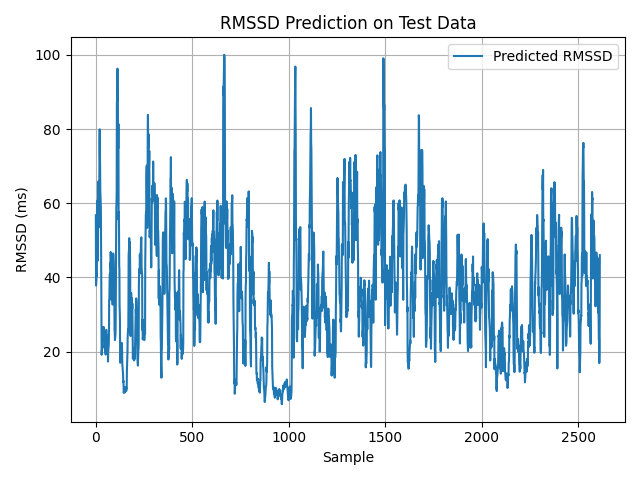
\includegraphics[width=0.67\textwidth]{rmsd_prediction.png}
    \caption{Przewidywane wartości RMSSD przez model}
\end{figure}
\begin{figure}[h]
    \centering
    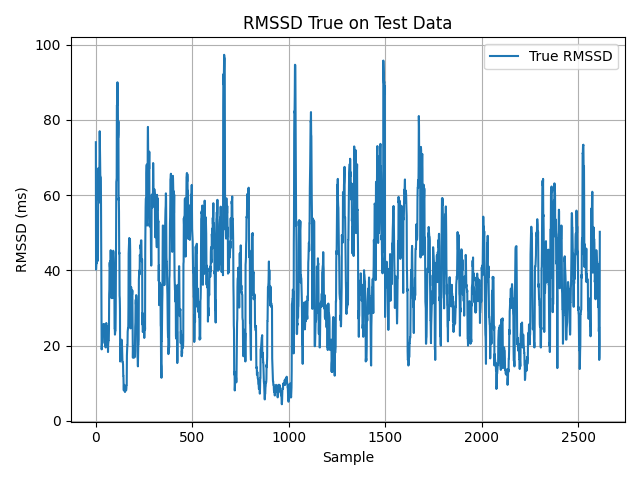
\includegraphics[width=0.67\textwidth]{rmsd_true.png}
    \caption{Rzeczywiste wartości RMSSD wyliczone na podstawie sygnału}
\end{figure}
\newpage
\begin{figure}[h]
    \centering
    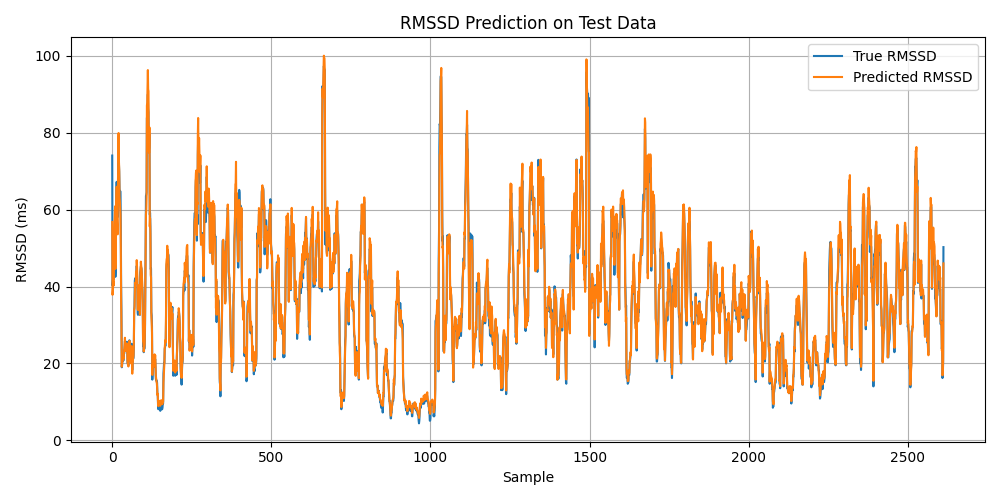
\includegraphics[width=0.7\textwidth]{rmssd_combinded.png}
    \caption{ Bezpośrednie porównanie wartości przewidywanych i rzeczywistych}
\end{figure}
Estymowane przez model wartości RMSSD cechują się bardzo wysoką zgodnością z wartościami rzeczywistymi. Model skutecznie odwzorowuje zarówno trend zmian, jak i dynamikę sygnału w tym gwałtowne spadki oraz lokalne maksima. Świadczy to o dobrej predykcji w odniesieniu do nowych, nieznanych danych.
Do ilościowej oceny jakości działania modelu wykorzystano metrykę błędu średniokwadratowego (MSE). Uzyskany błąd testowy był niski, co potwierdza skuteczność zastosowanej architektury oraz odpowiednio dobranych hiperparametrów treningowych.

\newpage
\section{Aplikacja do pomiaru tętna}
W ramach projektu opracowano aplikację mobilną na system Android umożliwiającą pomiar tętna z wykorzystaniem fotopletyzmografii (PPG). Aplikacja rejestruje sygnał PPG za pomocą tylnej kamery smartfona oraz wbudowanej latarki, co pozwala na nieinwazyjne śledzenie pulsacji krwi w palcu użytkownika.

\subsection{Zasada działania}
Użytkownik uruchamia aplikację i przykłada opuszek palca do tylnej kamery telefonu. Latarka automatycznie oświetla skórę, a kamera rejestruje obraz, w którym zmiany intensywności światła odbitego od tkanek odpowiadają cyklicznym zmianom objętości krwi.

Na ekranie aplikacji wyświetlany jest wykres sygnału PPG w czasie rzeczywistym, co umożliwia obserwację zmian rytmu serca w trakcie trwania pomiaru. Dodatkowo użytkownik może ręcznie oznaczać momenty wdechu i wydechu za pomocą dedykowanego przycisku. Każde takie zdarzenie zapisywane jest do pliku razem z znacznikiem czasu, co umożliwia późniejszą analizę zależności między cyklem oddechowym a tętnem.

\begin{figure}[h]
    \centering
    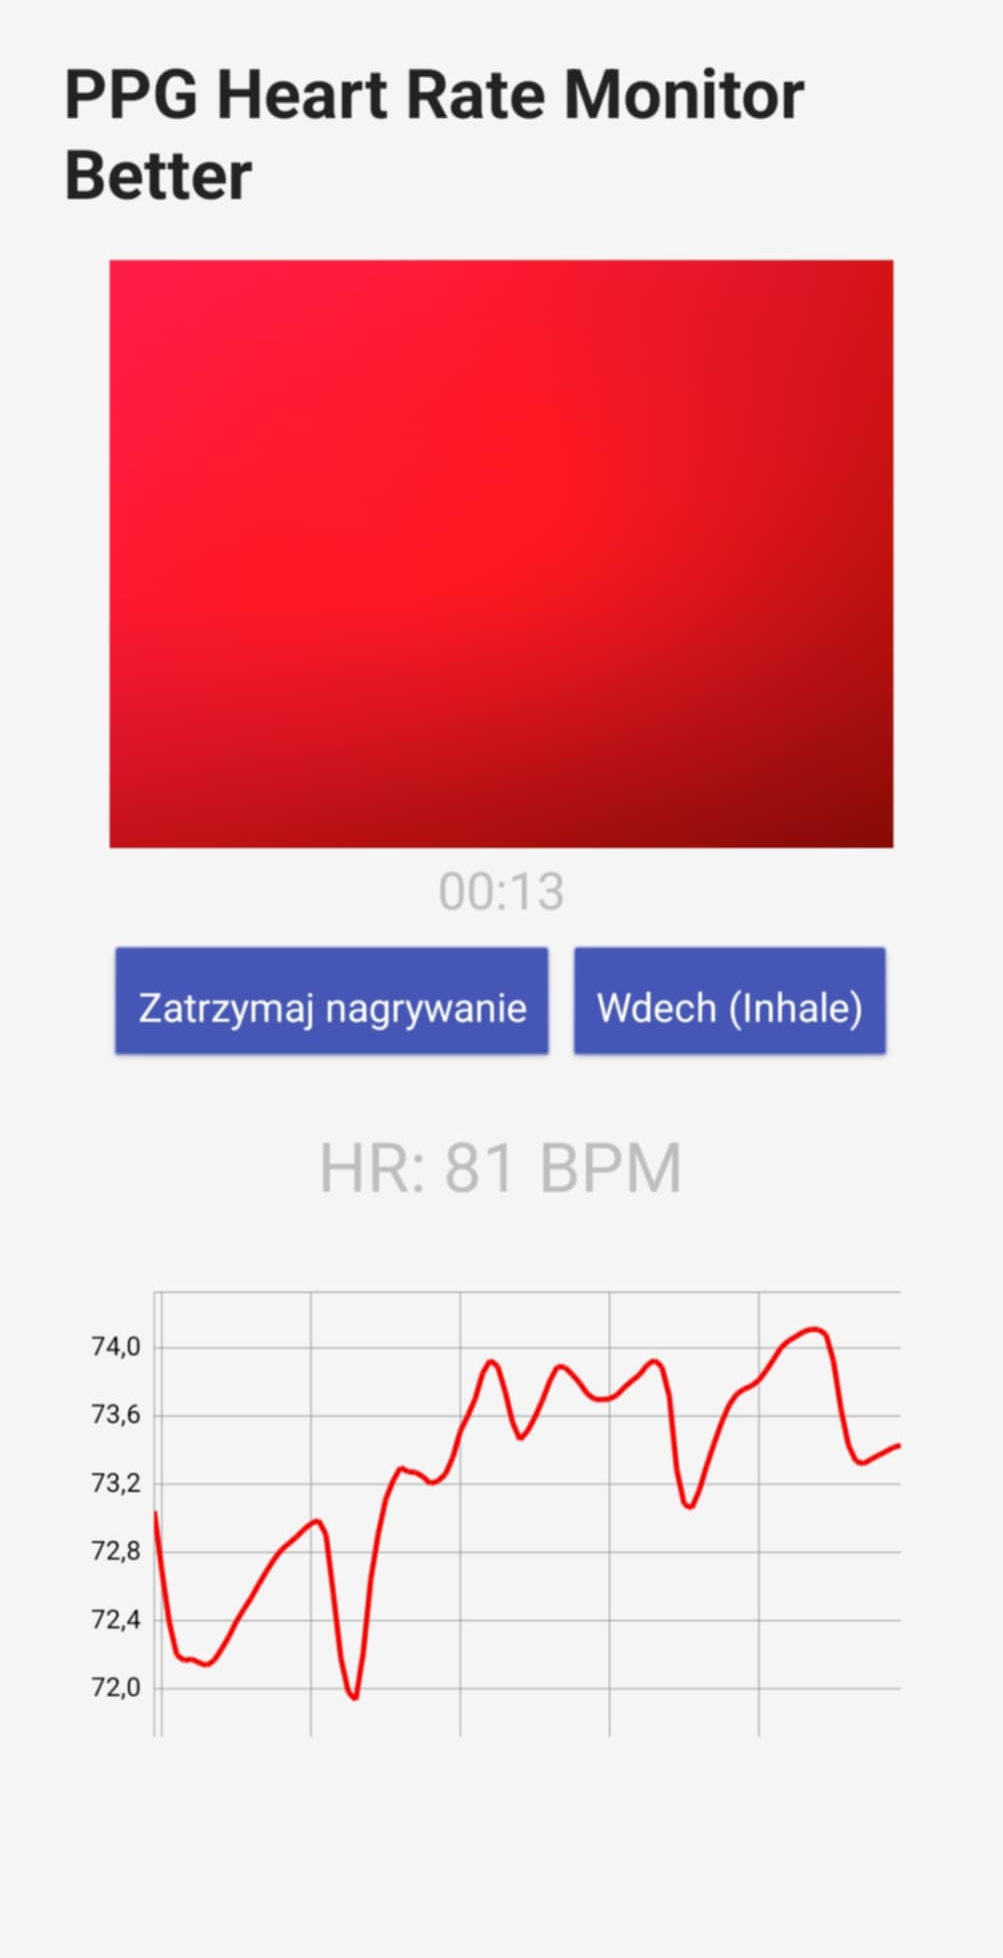
\includegraphics[scale=0.2]{aplikacja.png}
    \caption{Interfejs aplikacji mobilnej podczas pomiaru tętna }
\end{figure}
\newpage
\subsection{Przetwarzanie sygnału i obliczanie tętna}

Dla każdej klatki nagrania wideo aplikacja wyodrębnia zielony kanał, który najdokładniej odwzorowuje zmiany przepływu krwi. Obliczana jest średnia wartość jasności pikseli, co tworzy jednowymiarowy sygnał czasowy – sygnał PPG.

Sygnał ten jest filtrowany przy użyciu filtra dolnoprzepustowego w celu redukcji szumów. Na podstawie przefiltrowanego sygnału identyfikowane są lokalne maksima, które odpowiadają kolejnym uderzeniom serca. Różnice czasowe między tymi pikami pozwalają na wyznaczenie tętna (BPM) według wzoru:

\[
\text{BPM} = \frac{60}{\text{średni czas między pikami [s]}}
\]

Wynik jest aktualizowany dynamicznie w trakcie trwania pomiaru, a dane — w tym wartości sygnału PPG oraz oznaczenia wdechów i wydechów — zapisywane są do pliku w celu dalszej analizy.

\newpage
\section{Porównanie pomiaru tętna za pomocą aplikacji mobilnej i urządzenia Polar}
W celu porównania dokładności pomiaru tętna przeanalizowano dane pochodzące z dwóch źródeł: apli-
kacji mobilnej wykorzystującej sygnał PPG oraz urządzenia Polar, którego zapis EKG został poddany
analizie za pomocą algorytmu AI opartego na detekcji szczytów R i technikach przetwarzania sygnałów.

\subsection{Pierwszy pomiar}
\begin{figure}[h]
    \centering
    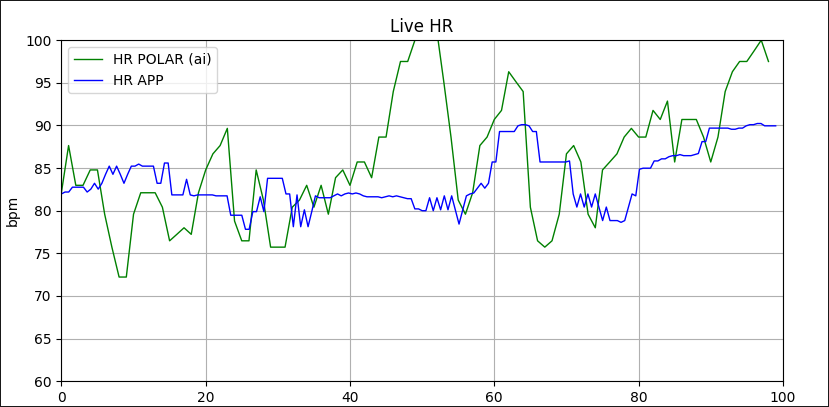
\includegraphics[width=0.67\textwidth]{image-5.png}
    \caption{Zestawienie HR: aplikacja mobilna a urządzenie Polar z algorytmem AI}
\end{figure}

Na pierwszym wykresie widoczna jest wyraźna różnica między przebiegiem tętna uzyskanego z aplikacji mobilnej a pomiarem EKG z urządzenia Polar. Aplikacja generuje bardziej wygładzony i stabilny sygnał, z wartościami tętna w wąskim zakresie 80–85 bpm. W przeciwieństwie do niej, metoda oparta na detekcji szczytów R wykazuje większą zmienność rytmu, z wahaniami od około 75 do 100 bpm. Pomiar EKG dokładniej odwzorowuje krótkoterminowe zmiany fizjologiczne, ale może być bardziej podatny na zakłócenia. Zauważalny wzrost tętna w przedziale 40–60 sekundy może wynikać z chwilowego wysiłku fizycznego lub zmiany pozycji ciała.

\newpage
\subsection{Drugi pomiar}
\begin{figure}[h]
    \centering
    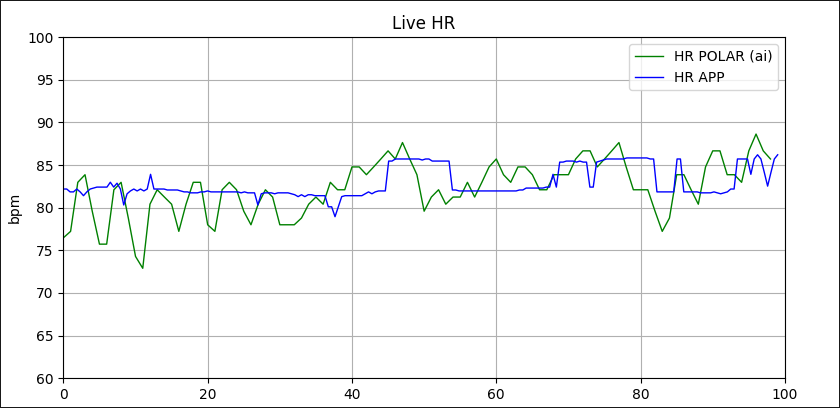
\includegraphics[width=0.67\textwidth]{image-4.png}
    \caption{Zestawienie HR: aplikacja mobilna a urządzenie Polar z algorytmem AI}
\end{figure}

Na drugim wykresie przedstawiono dane z innego okresu rejestracji, w którym badana osoba pozostawała w spoczynku. Oba przebiegi, z aplikacji mobilnej oraz z  urządzenia Polar, wykazują większą zbieżność. Wartości tętna mieszczą się w węższym zakresie, od 80 do 85 uderzeń na minutę, choć w sygnale uzyskanym metodą opartą na detekcji szczytów R nadal widoczna jest nieco większa zmienność. Mniejsze różnice między metodami sugerują, że w stabilnych warunkach ich dokładność może być porównywalna. Mimo to EKG pozostaje bardziej precyzyjne w rejestrowaniu krótkoterminowych wahań rytmu serca.

\subsection{Obserwacje}
Pomiar tętna z wykorzystaniem aplikacji mobilnej opartej na PPG charakteryzuje się większą stabilnością sygnału, ze względu na wygładzenia sygnału oraz mniejszą wrażliwość na krótkotrwałe wahania. Natomiast metoda oparta na analizie sygnału EKG dla urządzenia Polar cechuje się większą reaktywnością, skutkując bardziej dynamicznym przebiegiem sygnału, ale również większą podatnością na zakłócenia. W zależności od przyjętego celu, ogólnego monitorowania parametrów życiowych lub analizy krótkoterminowych zmian, każda z metod wykazuje odmienne zalety i ograniczenia.

\newpage
\section{Podsumowanie i wnioski}
% \subsection{Kluczowe obserwacje}
% \subsection{Wnioski końcowe}
Pokazane zostało, że połączenie konwolucyjnych sieci neuronowych z rekurencyjnymi warstwami typu LSTM umożliwia skuteczną detekcję istotnych elementów sygnału EKG, takich jak załamki R, co może posłużyć jako podstawa do dalszej analizy HRV i powiązań z rytmem oddechowym.

Przeprowadzone eksperymenty potwierdziły, że możliwe jest nieinwazyjne monitorowanie zależności między pracą serca a oddechem z użyciem nowoczesnych czujników i metod sztucznej inteligencji. Dzięki integracji danych z różnych źródeł (EKG i PPG), możliwe jest uzyskanie pełniejszego obrazu stanu fizjologicznego człowieka, co może mieć istotne znaczenie w diagnostyce i monitoringu stanu zdrowia.

\end{document}